\section{Функция Грина для задачи Дирихле (случай $\R^3$). Функция Грина для шара. Формула Пуассона решения задачи Дирихле для уравнения Лапласа в шаре}
% Затехал: Дмитрий Федоряка

\Subsection{Функция Грина}
Пусть $\Omega \subset \R^3$ - ограниченная область с кусочно-гладкой границей.

Пусть $u(x) \in C^2(\Omega) \cap C^1(\overline{\Omega})$ --- некоторое классическое решение задачи:

\[\begin{cases}
   \triangle u = f(x), & x\in \Omega \\
   \while{u}{\partial \Omega} = u_0(x), & x \in \partial \Omega  
\end{cases}\]  

Запишем интегральное представление:

$$ u = \int_{\Omega}{\roundBr{\frac{-1}{4 \pi |x-y|}}  {\triangle u(y)} dy} - \oint_{\partial \Omega}{\roundBr{\frac{-1}{4 \pi |x-y|}} \frac{\partial u(y)}{\partial \overrightarrow{n}_y} d S_y} + 
\oint_{\partial \Omega}{ {u(y)} \frac{\partial}{\partial \overrightarrow{n}_y}\roundBr{\frac{-1}{4 \pi |x-y|}}d S_y}
$$

Рассмотрим задачу при фиксированном $x \in \Omega$:

\[\begin{cases}
   \triangle_y g(x,y) = 0, & \Forall y \in \Omega \\
   g(x,y)|_{\partial \Omega} = \frac{1}{4 \pi |x-y|}  
\end{cases}\] 

Если $\partial \Omega \in C^2$, то решение существует (пока не можем это доказать).

Используем вторую формулу Грина:

$$ \int_{\Omega}{\triangle_y u(y) g(x,y)dy} - 
{\underset{=0}{\int_{\Omega}{u(y) \triangle_y g(x,y) dy}}}=$$

$$=\oint_{\partial \Omega} {\frac{\partial u(y)}{\partial \overrightarrow{n}_y} g(x,y) dS_y} - \oint_{\partial \Omega} {\frac{\partial g(x,y)}{\partial \overrightarrow{n}_y} u(y) dS_y} $$

Отсюда получаем

$$\int_{\Omega}{g(x,y) f(y) dy} + \underset{wanted~to~find}{\oint_{\partial \Omega}{\roundBr{\frac{-1}{4 \pi |x-y|}} \frac{\partial u(y)}{\partial \overrightarrow{n}_y} d S_y}}+ \oint_{\partial \Omega}
{\frac{\partial g(x,y)}{\partial \overrightarrow{n}_y}u(y) dS_y} = 0
$$

Тогда

$$u(x) = \int_{\Omega} {\roundBr{\frac{-1}{4 \pi |x-y|} +g(x,y)} f(y) dy} + \oint_{\partial \Omega} {u_0(y) \frac{\partial}{\partial \overrightarrow{n}_y} \roundBr{\frac{-1}{4 \pi |x-y|}+g(x,y)}dS_y}
$$

\textbf{Функция Грина}, по определению:

$$G(x,y) \triangleq  \frac{-1}{4 \pi |x-y|} + g(x,y) $$

Она симметрична и имеет ту же особенность, что и $\frac{-1}{4 \pi |x-y|}$





\Subsection{Функция Грина для шара}


Получим функцию Грина для шара:
\[\begin{cases}
   \triangle_y g(x,y) = 0, y \in \Omega \\
   g(x,y)|_{|y|=R} = \frac{1}{4 \pi |x-y|}& 
\end{cases}\]  

Будем обозначать $x^*$ точку, инверсную точке $x$ относительно окружности $|y|=R$.
$$x^* = x \frac{R^2}{|x|^2}$$
\begin{center}
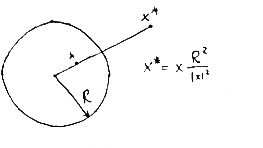
\includegraphics{20_1_new}
\end{center}
Покажем, что решением является функция:

\[g(x,y) = \begin{cases}
   \frac{R}{4 \pi |x| |y-x^*|},   & x \ne 0 \\
   \frac{1}{4 \pi R},& x=0
\end{cases}\]

Функция $g(x,y)$ - гармоническая по $y$ в шаре $|y|<R$ (особенность $y=x^*$ лежит вне шара, т.к. $x*$ лежит внутри него).

Посмотрим значение функции $g$ на границе:
\begin{center}
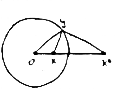
\includegraphics{20_2_new}
\end{center}
Заметим, что $\triangle OXY \sim \triangle OYX*$, т.к. $\angle XOY$- общий, и $\frac{|x|}{|y|}  =\frac{|y|}{|x^*|}$.

Из подобия $\frac{|y-x|}{|y-x^*} = \frac{|x|}{|y|} = \frac{|x|}{R}$.

Значит, $\left.\frac{R}{4 \pi |x| |y-x^*|} \right|_{|y|=R} = \frac{1}{4 \pi y}$, что и требовалось.

\Subsection{Формула Пуассона в шаре}

Получим формулу Пуассона решения задачи Дирихле в шаре:

$$u(x) = \int_{\Omega}{G(x,y) \underset{=0}{f(y)} dy} +
\oint_{\partial \Omega}{u_0(y) \frac{\partial G(x,y)}
{\partial \overrightarrow{n}_y}dS_y}
$$
Преобразуем последний интеграл:\\

$
\frac{\partial G(x,y)}{\partial \overrightarrow{n}_y}=
\sum_{k=1}^{3}{n_k(y) \left. \frac{\partial G}{\partial y_k} \right|_{|y|=R}}=
\sum_{k=1}^{3}{n_k(y)\frac{\partial}{\partial y_k}\left[
-\frac{1}{4\pi}\left(\frac{1}{|y-x|}-\frac{R}{|x|}\frac{1}{|y-x^*|}\right)
\right]} 
=
\frac{1}{4 \pi}  \sum_{k=1}^{3}\underset{=n_k(y)}{\frac{y_k}{R}}\left[ \frac{y_k-x_k}{|y-x|^3} - \frac{R}{|x|}  \frac{y_k-x_k^*}{|y-x^*|^3} \right]
$\\

Вспомним, что $\left.\frac{R}{|x|\cdot|y-x^*|}\right|_{|y|=R} =
\frac{1}{|x-y|}$:

$$
\left. \frac{\partial G(x,y)}{\partial \overrightarrow{n}_y} \right|_{|y|=R} 
=
\sum_{k=1}^{3}{\frac{1}{4 \pi} \frac{y_k}{R}
\left[ \frac{y_k-x_k}{|y-x|^3} -\frac{R}{|x|}\roundBr{\frac{|x|}{R}}^3
\frac{y_k - x_k^*}{|y-x|^3} \right] }
=
\frac{1}{4 \pi R |y-x|^3} \sum_{k=1}^{3}{y_k \squareBr{y_k-x_k-\frac{|x|^2}{R^2}(y_k - x_k^*)}}
=
$$

$$
=
\frac{1}{4 \pi R |y-x|^3} \squareBr{\angleBr{y,y-x} - \frac{|x|^2}{R^2}
\angleBr{y,y-x^*}}
=
\frac{1}{4 \pi R |y-x|^3} \squareBr{\underset{=R^2}{\angleBr{y,y}} - \angleBr{y,x}
-\frac{|x|^2}{R^2}\underset{=R^2}{\angleBr{y,y}}+ \underset{=\angleBr{y,x}}{\frac{|x|^2}{R^2} \angleBr{y,x^*}}  }
= $$ 
$$
=\frac{R^2 - |x|^2}{4 \pi R |y-x|^3}
$$

Итак, \textbf{формула Пуассона для решения задачи Дирихле для уравнения Лапласа в шаре}:

$$
u(x) = \frac{1}{4 \pi R} \oint_{|y|=R}{\frac{R^2-|x|^2}{|y-x|^3}u_0(y) dS_y}
$$


